
\documentclass[main.tex]{subfiles}
\begin{document}

\chapter{Derivation of the Flow Coefficients}
\label{outflows:sec:coefficients-derivation}

\begin{figure}
\centering
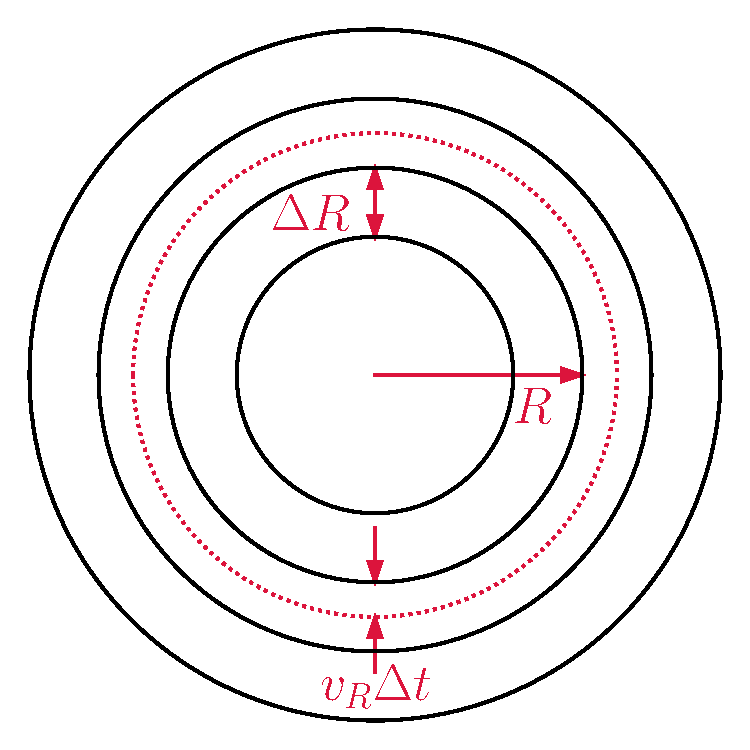
\includegraphics[scale = 0.5]{chapter7/schematic.pdf}
\caption{
A schematic of our derivation of the flow coefficients~$\mu_\flow$
and~$\gamma_\flow$.}
\label{outflows:fig:coefficients-schematic}
\end{figure}

\begin{itemize}

	\item The goal is to motivate a parameterization that includes the effect
	of radial gas flows in one-zone GCE models.
	Here we present the derivation of the coefficients~$\mu_\flow$ and
	$\gamma_\flow$ introduced in~\S~X.Y.Z.

	\item Consider a ring embedded in the Milky Way disk spanning the radial
	range~$R \rightarrow R + \Delta R$ which is described by a one-zone model.
	In the limit of a single, uniform inward flow velocity~$v_R$, all of the
	ISM material in the range~$R \rightarrow R + v_R \Delta t$ will be lost
	to the next ring inward in one differential timestep of size~$\Delta t$.
	Fig.~\ref{outflows:fig:coefficients-schematic} shows a schematic of this
	spatial configuration.
	The mass that migrates inward can then be expressed according to the
	area fraction~$a$ given by
	\begin{equation}\begin{split}
	a &\equiv \frac{
		\pi \left(R + v_R \Delta t\right)^2 - R^2
	}{
		\pi \left(R + \Delta R\right)^2 - R^2
	}
	\\
	&= \frac{
		2 R v_R \Delta t + v_R^2 \Delta t^2
	}{
		2 R \Delta R + \Delta R^2
	}.
	\label{outflows:eq:area-frac-def}
	\end{split}\end{equation}
	Simultaneously, material will be gained from the next ring out, spanning
	radii~$R + \Delta R \rightarrow R + 2\Delta R$.
	The net flow rate of some element~$x$ can then be expressed as the
	difference of these two source and sink terms:
	\begin{equation}\begin{split}
	\dot{M}_{x,\flow} &= \dot{M}_{x,\flow,\text{in}} -
	\dot{M}_{x,\flow,\text{out}}
	\\
	&= Z_x(R + \Delta R) M_g(R + \Delta R) \frac{a(R + \Delta R)}{\Delta t} -
	Z_x(R) M_g(R) \frac{a(R)}{\Delta t},
	% \\
	% &= Z_x(R) M_g(R) \frac{a(R)}{\Delta t}
	% \left(
	% \frac{Z_x(R + \Delta R)}{Z_x(R)}
	% \frac{M_g(R + \Delta R)}{M_g(R)}
	% \frac{a(R + \Delta R)}{a(R)}
	% - 1\right)
	\label{outflows:eq:flowin-minus-flowout}
	\end{split}\end{equation}
	where~$Z_x \equiv M_x / M_g$ is the mass-fraction of the element~$x$ in the
	ISM and~$M_g$ is the mass of the ISM gas itself.
	We clarify that for the sake of this derivation, we define an inward
	velocity to have positive sign (i.e.,~$v_R > 0$) so that we do not have to
	keep track of an additional minus sign for notational convenience.
	We then apply a~$v_R \rightarrow -v_R$ transformation at the end in order
	for~$v_R > 0$ to correspond to an outward radial velocity according to
	convention.

	\item Regardless of the functional form of~$Z_x(R)$ and~$M_g(R)$, they can
	be expressed in terms of a Taylor series, along with~$a$:
	\begin{subequations}\begin{align}
	Z_x(R + \Delta R) &= Z_x(R) +
	\sum_{i = 1}^\infty \frac{\partial^i Z_x}{\partial R^i} \Delta R^i
	\\
	M_g(R + \Delta R) &= M_g(R) +
	\sum_{i = 1}^\infty \frac{\partial^i M_g}{\partial R^i} \Delta R^i
	\\
	a(R + \Delta R) &= a(R) +
	\sum_{i = 1}^\infty \frac{\partial^i a}{\partial R^i} \Delta a^i.
	\end{align}\end{subequations}
	Although it is straightforward to evaluate~$a(R + \Delta R)$ with the
	transformation~$R \rightarrow R + \Delta R$ in
	equation~\refp{outflows:eq:area-frac-def}, it is notationally convenient to
	this derivation to write it in terms of a Taylor expansion.
	Plugging these expressions into
	equation~\refp{outflows:eq:flowin-minus-flowout}:
	\begin{equation}\begin{split}
	\dot{M}_{x,\flow} &= Z_x(R) M_g(R)
	\frac{2 R v_R + v_R^2 \Delta t}{2 R \Delta R + \Delta R^2}
	\Bigg[
	\left(1 + \frac{1}{Z_x(R)}
	\sum_{i = 1}^\infty \frac{\partial^i Z_x}{\partial R^i} \Delta R^i\right)
	\\
	&\quad
	\left(1 + \frac{1}{M_g(R)}
	\sum_{i = 1}^\infty \frac{\partial^i M_g}{\partial R^i} \Delta R^i\right)
	\left(1 + \frac{1}{a(R)}
	\sum_{i = 1}^\infty \frac{\partial^i a}{\partial R^i} \Delta R^i\right)
	- 1\Bigg].
	\end{split}\end{equation}

	\item At this point, we take the limit of the above expression as
	$\Delta R$ and $\Delta t \rightarrow 0$ to parameterize the flow rate in a
	manner that is independent of these arbitrary choices of the ring width and
	the timestep size.
	For notational convenience, we let~$\Gamma$ denote the quantity in square
	brackets:
	The limit as~$\Delta t \rightarrow 0$ is trivial:
	\begin{equation}
	\lim_{\Delta t \rightarrow 0} \dot{M}_{x,\flow} = Z_x(R) M_g(R)
	\frac{2 R v_R}{2 R \Delta R + \Delta R^2} \Gamma,
	\end{equation}
	but the limit as~$\Delta R \rightarrow 0$ requires L'H\^opital's Rule since
	both~$2 R \Delta R + \Delta R^2$ and~$\Gamma \rightarrow 0$.
	Taking the derivative of~$\Gamma$ with respect to~$\Delta R$ to this end:
	\begin{subequations}\begin{align}
	\lim_{\Delta R \rightarrow 0} \dot{M}_{x,\flow} &=
	Z_x(R) M_g(R) \left( \frac{2 R v_R}{2R + 2 \Delta R} \right)
	\frac{\partial \Gamma}{\partial \Delta R}
	\\
	\begin{split}
	\frac{\partial \Gamma}{\partial \Delta R} &=
	\left(\frac{1}{Z_x} \sum_{i = 1}^\infty i
	\frac{\partial^i Z_x}{\partial R^i} \Delta R^{i - 1}\right)
	\left(1 + \frac{1}{M_g(R)}
	\sum_{i = 1}^\infty \frac{\partial^i M_g}{\partial R^i} \Delta R^i\right)
	\\
	&\quad
	\left(1 + \frac{1}{a(R)}
	\sum_{i = 1}^\infty \frac{\partial^i a}{\partial R^i} \Delta R^i\right) +
	\\
	&\quad
	\left(1 + \frac{1}{Z_x(R)}
	\sum_{i = 1}^\infty \frac{\partial^i Z_x}{\partial R^i} \Delta R^i\right)
	\left(\frac{1}{M_g} \sum_{i = 1}^\infty i
	\frac{\partial^i M_g}{\partial R^i} \Delta R^{i - 1}\right)
	\\
	&\quad
	\left(1 + \frac{1}{a(R)}
	\sum_{i = 1}^\infty \frac{\partial^i a}{\partial R^i} \Delta R^i\right) +
	\\
	&\quad
	\left(1 + \frac{1}{Z_x(R)}
	\sum_{i = 1}^\infty \frac{\partial^i Z_x}{\partial R^i} \Delta R^i\right)
	\left(1 + \frac{1}{M_g(R)}
	\sum_{i = 1}^\infty \frac{\partial^i M_g}{\partial R^i} \Delta R^i\right)
	\\
	&\quad
	\left(\frac{1}{a} \sum_{i = 1}^\infty i \frac{\partial^i a}{\partial R^i}
	\Delta R^{i - 1}\right).
	\end{split}
	\end{align}\end{subequations}
	Since we are taking the limit as~$\partial \Gamma / \partial \Delta R$
	approaches zero, despite the complicated nature of its expression, all but
	terms with~$\Delta R^{i - 1}$ with~$i = 1$ drop out entirely.
	Furthermore, it is straight-forward to demonstrate that~$(1 / a) \partial a
	/ \partial R \rightarrow 0$ in the limit that $\Delta t, \Delta R
	\rightarrow 0$.
	This results in the following expression for~$\dot{M}_{x,\flow}$:
	\begin{equation}
	\dot{M}_{x,\flow} = Z_x(R) M_g(R) v_R \left(
	\frac{1}{Z_x} \frac{\partial Z_x}{\partial R} +
	\frac{1}{M_g} \frac{\partial M_g}{\partial R}
	% \frac{1}{a} \frac{\partial a}{\partial R}
	\right).
	\label{outflows:eq:mdot-flow-general}
	\end{equation}

	\item At this point, we derive expressions for~$(1 / Z_x) \partial Z_x /
	\partial R$ and~$(1 / M_g) \partial M_g / \partial R$ appropriate for a
	disk galaxy like the Milky Way in an equilibrium state as suggested by
	the results in~\S~\ref{outflows:sec:empirical}.

	\item For a linear gradient in [X/H] of slope~\grad{X}, the abundance by
	mass of the element~$x$ is an exponential
	\begin{equation}
	Z_x = Z_{x,\odot} e^{-(R - R_\odot) / R_x},
	\end{equation}
	where~$R_\odot \approx 8$ kpc is the Galactocentric radius of the sun,
	$Z_{x,\odot}$ is the abundance by mass of~$x$ in the sun, and
	$R_x \equiv -(\grad{X} \ln 10)^{-1}$ is the scale radius implied by the
	slope of the [X/H] gradient.
	In this case, the derivative of~$Z_x$ with respect to radius is trivial:
	\begin{equation}
	\frac{\partial Z_x}{\partial R} = \frac{-Z_x}{R_x}.
	\label{outflows:eq:partial-zx-radius}
	\end{equation}

	\item The mass in a given ring changes with radius not only due to the
	exponential decline of surface density but also due to the increasing area
	of the ring:
	\begin{equation}\begin{split}
	\frac{\partial M_g}{\partial R} &= \frac{\partial}{\partial R}
	\left(2 \pi R \Delta R \Sigma_{g,0} e^{-R / R_g}\right)
	\\
	&= 2 \pi \Delta R \Sigma_{g,0} \left(e^{-R / R_g} - \frac{R}{R_g}
	e^{-R / R_g}\right)
	\\
	&= M_g(R) \left(\frac{1}{R} - \frac{1}{R_g}\right),
	\label{outflows:eq:partial-mgas-radius}
	\end{split}\end{equation}
	where~$\Sigma_{g,0}$ is simply a constant of normalization for the
	exponential gas disk and~$R_g$ is some scale radius.

	\item Plugging equations~\refp{outflows:eq:partial-zx-radius}
	and~\refp{outflows:eq:partial-mgas-radius} into equation
	\refp{outflows:eq:mdot-flow-general} yields
	\begin{equation}
	\dot{M}_{x,\flow} = -Z_x \dot{M}_\star \tau_\star v_R
	\left(\frac{1}{R} - \frac{1}{R_g} - \frac{1}{R_x}\right)
	\end{equation}
	as the expression for the flow rate of some element~$x$ if the Galactic
	disk is in chemical equilibrium and the scale radius of the ISM surface
	density is not changing significantly with time.
	In the above expression, we have now applied the~$v_R \rightarrow -v_R$
	transformation so that~$v_R > 0$ corresponds to an~\textit{outward} flow.
	For the sake of including this term in GCE models, it is useful to express
	the rate in terms of the SFR, so we have substituted in the SFE timescale
	$\tau_\star \equiv M_g / \dot{M}_\star$.

	\item The flow rate of~\textit{gas} follows a similar derivation, and can
	be deduced from the above expressions if one simply sets~$Z_x = 1$
	everywhere.
	The gas flow rate is then given by
	\begin{equation}
	\dot{M}_{g,\flow} = -\dot{M}_\star \tau_\star v_R
	\left(\frac{1}{R} - \frac{1}{R_g}\right).
	\end{equation}

	\item We now introduce the unitless coefficients~$\mu_\flow$
	and~$\gamma_\flow$
	\begin{subequations}\begin{align}
	\mu_\flow &\equiv -\tau_\star v_R
	\left(\frac{1}{R} - \frac{1}{R_g} - \frac{1}{R_x}\right)
	\\
	\gamma_\flow &\equiv -\tau_\star v_R
	\left(\frac{1}{R} - \frac{1}{R_g}\right) =
	\mu_\flow - \frac{\tau_\star v_R}{R_x}
	\end{align}\end{subequations}
	such that the rates of change of the metal and ISM gas masses can then be
	expressed as
	\begin{subequations}\begin{align}
	\dot{M}_{x,\flow} &= Z_x \dot{M}_\star \mu_\flow
	\\
	\dot{M}_{g,\flow} &= \dot{M}_\star \gamma_\flow.
	\end{align}\end{subequations}

	\item {\color{red} Further discussion of~$\mu_\flow$ and~$\gamma_\flow$
	probably belongs in the main text of the paper, though this Appendix will
	need some sort of brief conclusion.}

\end{itemize}

\end{document}

